\documentclass[fr]{../../../eplsummary}

\usepackage{../../../eplelec}
\usepackage{../../../eplunits}

\usepackage{pgfplots}
\usepackage{circuitikz}
\usepackage{subcaption}

\newtheorem{defin}{Definition}[section]
\newtheorem{nota}[defin]{Notation}
\newtheorem{prop}[defin]{Propriete}

%%Tres Draft je sais... %%
%\setlength{\parindent}{0em} % Vire les alinéas
%\setlength{\parskip}{0.6em} % Agrandit l'espace entre les paragraphs

\hypertitle[']{\'Electronique}{2}{FSAB}{1202}
{Nicolas Cognaux\and Beno\^it Legat\and Lucas Nyssens\and Antoine Paris}
{Piotr Sobieski}

\part{Électromagnétisme}

\section{Champ magnétique}
Un champ magnétique $\B$ est un champ créé par un déplacement de charge
(selon la loi de Biot-Savart, voir \sectionref{bs})
qui provoque une force sur les charges en mouvement
(c'est la force de Lorentz, voir \sectionref{lorentz}).

A l'intérieur d'un aimant, les lignes de champ vont du Sud au Nord.
A l'extérieur, les lignes de champs vont du Nord au Sud.
{\bf Il n'y a jamais de monopôle magnétique !}

Le pôle Nord d'un aimant pointe vers le pôle Nord géographique
qui est le pôle Sud magnétique.

$B$ (exprimé en $\tesla$) est l'induction magnétique et $H$ (exprimé en $\ampere\per\meter$)
le champ magnétique.
On a la relation
\[ B = \mu_0\mu_rH \]
où $\mu_0$ est la perméabilité du vide,
elle vaut $\unit{4\pi \cdot 10^{-7}}{\tesla\meter\per\ampere}$.
À chaque fois qu'on utilisera $\mu_0$ sans $\mu_r$,
on considérera qu'on est dans le vide.
Si la formule doit être utilisée dans un matériau avec un certain $\mu_r$,
il suffit de remplacer $\mu_0$ par $\mu_0\mu_r$.
Attention néanmoins,
si on est dans le cas d'un matériau ferromagnétique qui se magnétise
(i.e. $H$ varie), $\mu_r$ n'est pas constant !
Plus d'info à la \sectionref{ferro}.

\section{Flux}
Le flux électrique d'un champ électrique $E$
à travers une surface orientée $S$ vaut
\[ \Phi_E = \int \E \cdot \dif \vec S. \]
Le flux magnétique d'un champ magnétique $B$
à travers une surface orientée $S$ vaut
\[ \Phi_B = \int \B \cdot \dif \vec S. \]
L'unité de $\Phi_B$ est le $\weber = \tesla \cdot \meter \squared$.

% Pas sur que ce soit tout à fait correcte.
%\paragraph{Remarque}
%Le flux rentrant dans un volume est compté comme négatif tandis
%que le flux sortant est compté comme positif.

\section{Loi de Gauss}
L'intégrale du champ sur une surface fermée entourant un volume
\[ \oiint \B \cdot \dif \vec S = 0 = \Phi. \]
C'est dû au fait qu'un monopôle magnétique isolé n'existe pas.
Plus d'explication à l'\annexeref{gauss}.
\paragraph{Conséquences}
\begin{itemize}
  \item Les lignes de champs se bouclent sur elles-mêmes;
  \item Conservation du flux magnétique;
  \item Le flux magnétique revient du pôle Sud
    au pôle Nord en traversant l'aimant.
\end{itemize}

\section{Force de Lorentz}
\label{sec:lorentz}
Un courant est un déplacement de charges.
Si ce courant rencontre un champ magnétique $\B$ et un champ électrique $\E$,
il y a création d'une force:
\[ \vec F = q \E + q \vec v \times \B. \]
On l'appelle la force de Lorentz. Sa direction est celle donnée par la règle de
main droite pour une charge positive, et l'opposé de celle donnée par la règle
de la main droite pour une charge négative.

\paragraph{Remarques}
\begin{itemize}
  \item Par définition du produit vectoriel, $\vec v \perp \vec v \times \B$,
    donc $W = \vec v \cdot q\vec v \times \B = 0$.
    C'est à dire que le champ magnétique ne peut que changer
    la \textbf{direction} d'une particule chargée,
    \textbf{pas} la \textbf{norme} de sa \textbf{vitesse}.
\end{itemize}

\subsection{Applications de la force de Lorentz}
\subsubsection{Force sur un fil parcouru par un courant}
Dans le cas d'un courant circulant dans un champ, la formule devient
\[ \dif \vec F = I\dif \vec l \times \B. \]

\subsubsection{Force et couple sur une boucle}
Considérons une boucle de surface $S$ parcourue par un courant $I$
et un champ magnétique constant $\B$.
Soit $\vec S$, le vecteur surface ayant comme norme $S$,
normal à la surface de la boucle et dont le sens est déterminé
par le sens de $I$ et la règle de la main droite.
Soit
\footnote{$\vec \mu$ est aussi parfois noté $\vec m$.}
$\vec \mu = I \cdot \vec S$,
le moment dipolaire magnétique.
On peut calculer le torque exercé par le champ magnétique sur la boucle ainsi
\[ \vec \tau = \vec \mu \times \B. \]
On a aussi une énergie potentielle valant
\[ U = -\vec \mu \cdot \B = -\mu B \cos \phi \]
où $\phi$ est l'angle entre $\vec{B}$ et $\vec{\mu}$.
On voit ici que $\vec \mu$ et $\B$ tendent à s'aligner.
\begin{itemize}
  \item Si $\phi = 0$, $U = - \mu B$, c'est un équilibre stable,
    le niveau le plus bas d'énergie potentielle.
  \item Si $\phi = \pi$, $U = \mu B$, c'est un équilibre instable,
    le niveau le plus haut d'énergie potentielle.
    $\tau = 0$ mais il suffit d'un fifrelin pour que ça ne soit plus le cas.
\end{itemize}

Les forces parallèles à la surface de la boucle
(et donc perpendiculaires à sa normale $\vec{S}$) n'interviennent pas
dans la cinétique de la boucle.
Si elle est déformable,
elle se déformera jusqu'à atteindre une forme circulaire.
Une fois cette forme atteinte, elles s'annuleront entre elles.

\subsubsection{Moteur DC}
On peut donc utiliser la force de Lorentz pour créer un couple.
On utilise ça dans les moteurs électriques.
Un cadre est connecté à une borne + et une borne - par des balais.
Il tourne et quand il arrive à $\phi = 0$, il a encore un peu de vitesse,
donc il dépasse $\phi = 0$.
$\tau$ veut le ramener vers $\phi = 0$
car c'est le point de plus basse énergie potentielle.
Seulement, comme, il s'est retourné,
la partie du cadre connectée à la borne + est
maintenant connectée à la borne - et vice versa.
C'est à dire que le courant s'inverse,
le point de plus basse énergie devient donc $\phi = \pi$.
$\tau$ veut donc continuer dans le même sens mais arrivé en $\phi = \pi$,
il a encore un peu de vitesse, il dépasse donc $\phi = \pi$ et ainsi de suite.

\paragraph{Approximation utilisée}
Dans cette section, nous avons négligé le champ magnétique $\B$
généré par le courant $I$ passant dans la boucle.

\section{Loi de Biot-Savart}
\label{sec:bs}
Un courant crée un champ magnétique.
Ce champ est la somme vectorielle de tous les champs
générés par toutes les charges de ce courant.
Dans le \textbf{vide}, il vaut
\[ \dif\B = \frac{\mu_0}{4\pi}\frac{I\dif \vec l\times \hat r}{r^2}. \]
Il est important de noter que $||\hat r|| = 1$.
Il existe une autre version de la formule où on remplace $\hat r$ par
$\frac{\vec r}{r}$ et donc, au dénominateur,
$r^2$ devient $r^3$, ce qui revient au même.

\subsection{Applications de la loi de Bio-Savart}
\subsubsection{Champ sur l'axe d'une spire}
% Pour ce qui suit, faut-il indiquer la démonstration complète ?
% C'est sans doute mieux mais risque de prendre un peu de place.
Le champ à une distance $x$ sur l'axe d'une spire de rayon
$R$ traversée par un courant $I$ peut être calculé par Biot-Savart et vaut
\[ \B = \frac{\mu_0}{2}\cdot\frac{IR^2}{(R^2 + x^2)^{\frac{3}{2}}}. \]
Pour déterminer le champ au centre d'une spire, on utilise Biot-Savart.

\paragraph{Conséquences}
\begin{itemize}
  \item Le champ magnétique le long d'une bobine longue
    (pas infinie) n'est pas constant.
  \item Les bobines de Helmholtz sont des bobines espacées
    d'une distance $d = R$ où $R$ est le rayon des deux bobines.
    Cette configuration permet de générer un champ magnétique presque constant
    sur toute la longueur séparant les bobines
    comme vous pouvez le constater par la \figuref{deqr}.
\end{itemize}
\begin{figure}
  \begin{center}
    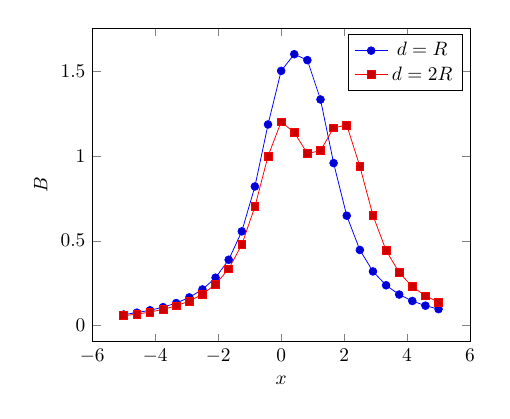
\begin{tikzpicture}[scale=0.7]
      \begin{axis}[xlabel=$x$, ylabel=$B$]
        \addplot {1/(1+x^2)+1/(1+(1-x)^2))};
        \addlegendentry{$d = R$}
        \addplot {1/(1+x^2)+1/(1+(2-x)^2))};
        \addlegendentry{$d = 2R$}
        \addlegendentry{une fonction}
      \end{axis}
    \end{tikzpicture}
  \end{center}
  \caption{$B$ dans l'axe de deux bobines espacées d'une distance $d$ où $R=1$}
  \label{fig:deqr}
\end{figure}

\section{Loi d'Ampère}
La loi d'Ampère dit que tout fil parcouru par un courant
est toujours entouré d'un champ magnétique.
Dans tout contour fermé,
\[ \oint \B \cdot \dif \vec l = \mu_0 I. \]

Pour déterminer le sens dans lequel faire l'intégrale,
il faut utiliser la règle de la main droite
où le pouce est le sens du courant
et les doigts dans la direction de $\dif\vec l$.

Seulement, la formulation précédente n'est vraie que dans le vide.
Il faut utiliser
\[ \oint \vec H \cdot \dif \vec l = I \]
dans les autres cas (dans le vide, $\B = \mu_0 \vec H$).

\paragraph{Remarque}
Pour que la formule marche dans tous les cas,
il faut introduire 3 types de courants:
$I_\mathrm{C}$, $I_\mathrm{D}$ et $I_\mathrm{M}$.
On définit alors
\[ I = I_\mathrm{C} + I_\mathrm{D} + I_\mathrm{M}. \]

\begin{itemize}
  \item Le premier est le courant électrique
    que nous connaissons qui est dû à un déplacement de charge.
    Dans la plupart des cas, considérer uniquement $I_\mathrm{C}$ suffit.
  \item Le second est le courant de déplacement qui vaut
    \[ I_\mathrm{D} = \perm_0\frac{\dif \Phi_E}{\dif t}. \]
    Par exemple, si on prend une boucle autour d'une capacité,
    il faut que $\mu_0I$ soit le même quand on passe par le fil et quand
    on passe entre les deux plaques donc il faut un courant entre les plaques.
    C'est $I_\mathrm{D}$ qui entre les deux plaques
    n'est pas nul qui établit l'égalité.
  \item Le troisième,
    le courant de magnétisation est un courant créé par un matériau magnétisé.
    Les orbitales de ses atomes, sous l'effet de la magnétisation,
    s'orientent et crée un courant microscopique.
    Il est très rare qu'on ne puisse pas le négliger à l'échelle macroscopique.
\end{itemize}
On a donc la loi d'Ampère généralisée par Maxwell
\[ \oint \B \dif \vec l =
\mu_0 \left(I_\mathrm{C} + \perm_0 \frac{\dif \Phi_E}{\dif t}\right). \]

\subsection{Applications de la loi d'Ampère}
\subsubsection{Champ dans un solénoïde long}
\label{sec:bbl}
\paragraph{Postulat}
\begin{itemize}
  \item $B_\mathrm{int}$ est constant et parallèle à l'axe de la bobine;
  \item $B_\mathrm{ext}$ est nul.
\end{itemize}
Par Ampère,
\begin{eqnarray*}
  B &=& \mu_0nI\\
  H &=& nI
\end{eqnarray*}
où $n$ est le nombre de spires par unité de longueur.
Pour la première équation, la bobine doit être dans le vide.
La deuxième équation gère les cas où la bobine n'est pas dans le vide.

\subsubsection{Champ dans un solénoïde toroïdal}
\label{sec:bst}
\paragraph{Postulat}
\begin{itemize}
  \item $B_\mathrm{int}$ est constant et tangent au tore;
  \item $B_\mathrm{ext}$ est nul.
\end{itemize}
Par Ampère,
\begin{eqnarray*}
  B &=& \mu_0\frac{NI}{2\pi r}\\
  H &=& \frac{NI}{2\pi r}
\end{eqnarray*}
où $N$ est le nombre de spires et $r$ le rayon moyen du tore,
c'est à dire la distance entre le centre du tore et le milieu d'une tranche.
Pour la première équation, la bobine doit être dans le vide.
La deuxième équation gère les cas où la bobine n'est pas dans le vide.

\subsubsection{Champ généré par un long fil}
\paragraph{Postulat}
\begin{itemize}
  \item $B$ est constant pour une même distance
    du fil et perpendiculaire au fil;
\end{itemize}
Par Ampère,
\[ \B = \frac{\mu_0I}{2\pi r} \]
où $r$ est la distance par rapport au fil.

Si on a deux fils parallèles à une distance $r$ l'un de l'autre, on a donc
\[ \dif F = \mu_0\frac{I_1I_2}{2\pi r}\dif l \]
où $F$ les attirent l'un à l'autre si le courant est
dans le même sens et les repoussent s'il est dans le sens contraire.

\subsubsection{Champ dans l'entrefer d'un électroaimant}
\paragraph{Postulat}
\begin{itemize}
  \item $H_e$ (dans l'entrefer) et $H_m$ (dans le matériau) sont constants ;
  \item $\mu_r \gg 1$.
\end{itemize}
Dans un électroaimant avec entrefer, la loi d'ampère devient :

\[ \oint \vec{H} \cdot \vec{dl} \approx LH_m + eH_e = NI\]

Où $e$ est la longueur de l'entrefer, $L$ la longueur du circuit magnétique, $N$
le nombre de spires de la bobine et $I$ le courant la parcourant.
Or, comme $\mu_r \gg 1$ (pour un matériau ferromagnétique par exemple) et que
tout le champ magnétisant se retrouve dans l'entrefer on a : $H_m \ll H_e$.
On peut donc calculer le champ dans l'entrefer :

\[ eH_e = NI \Rightarrow B_e = \mu_0\mu_r \frac{NI}{e} \]

On remarque que plus l'entrefer est petit, plus le champ dans l'entrefer est
fort.

\section{Inductance}
\subsection{Inductance mutuelle}
L'inductance mutuelle est un coéfficient permettant de décrire l'influence d'un circuit
magnétique sur un autre. Considèrons deux bobines dont la deuxième intercepte une partie
du flux variable produit par la première, on a par la loi de Lenz-Faraday (voir \sectionref{faraday}) :

\[ \EMF_2 = -N_2 \frac{\dif \Phi_2}{\dif t} \]

On peut réecrire cette équation en terme de proportionalité :

\[ N_2 \Phi_2 = M i_1 \]

Où $M$ est l'inductance mutelle. En dérivant cette expression, on obtient :

\[ N_2 \frac{\dif \Phi_2}{\dif t} = M \frac{\dif i_1}{\dif t} \Rightarrow \EMF_2 = -M \frac{\dif i_1}{\dif t} \]

Autrement dit : un changement du courant $i_1$ dans la première
bobine induit une différence de tension dans la deuxième bobine directement proportionnelle
au taux de variation de $i_1$. $M$ dépend de la taille, de la forme, du nombre de spires, de l'orientation,
de la distance séparant les bobines et des propriétés d'un éventuel matériau magnétique.
En résumé,

\[ M = N_2 \frac{\Phi_2}{i_1} = N_1 \frac{\Phi_1}{i_2} \]

\[ \EMF_1 = -M \frac{\dif i_2}{\dif t} \]

\[ \EMF_2 = -M \frac{\dif i_1}{\dif t} \]

\subsection{Inductance propre}
Dans l'inductance, chaque spire produit un champ magnétique et donc un flux.
Ce flux est intercepté par chaque spire et produit donc un courant
lors de la variation de ce flux
(selon la loi de Lenz-Faraday, voir \sectionref{faraday}).
On définit l'inductance comme suit
\[ L = N\frac{\Phi_B(I)}{I} \]
où $N$ est le nombre de spires et $\Phi_B(I)$
le flux dans \textbf{une seule} spire.
$\Phi_B(I)$ est proportionnel à $I$ donc $L$ ne dépend pas de $I$.

\subsection{Applications}
\subsubsection{Inductance dans un solénoïde long}
Comme vu à la \sectionref{bbl},
\[ B = \mu_0nI. \]
On a donc
\begin{align*}
  L &= N\frac{\Phi_B(I)}{I}\\
  &= \mu_0 nNS\\
  &= \mu_0 \frac{N^2}{l}S
\end{align*}
où $S$ est la surface d'une tranche du solénoïde et $l$ est sa longueur.

\subsubsection{Inductance dans un solénoïde toroïdal}
Comme vu à la \sectionref{bst},
\[ B = \mu_0\frac{NI}{2\pi r}. \]
On a donc
\begin{align*}
  L &= N\frac{\Phi_B(I)}{I}\\
  &= \mu_0 \frac{N^2}{2\pi r}S\\
  &= \mu_0 \frac{N^2}{2r}a^2
\end{align*}
où $S$ est la surface d'une tranche du solénoïde,
$r$ le rayon moyen du tore et $a$
le rayon d'une tranche (c'est à dire que $S = \pi a^2$).

\subsubsection{Transformateur}
\begin{center}
  \begin{circuitikz}[american voltages] \draw
    (0,0) node[transformer] (T) {}
    (T.B1) -| (3.5, 0) to[R, v=$V_2$, i = $I_2$] (3.5,-2) |- (T.B2)
    (T.A1) -| (-3.5, 0) to[sV, v=$V_1$, i = $I_1$] (-3.5,-2) |- (T.A2)
    (-1,-1) node{$N_1$}
    (1,-1) node{$N_2$}
    ;
  \end{circuitikz}
\end{center}

Dans un transformateur, une bobine crée un flux,
ce flux se déplace dans le noyau de ferrite
et est intercepté par une deuxième bobine.
Le transformateur ne fonctionne qu'en alternatif
car le flux doit être variable.

Par la conservation du flux, on a
\[ \frac{V_1}{V_2} = \frac{N_1}{N_2}. \]

Si on considère que le transformateur ne perd pas d'énergie, on a
\[ V_1I_1 = V_2I_2. \]
On utilise des lamelles comme noyau de ferrite pour éviter le
courants de foucault et donc les pertes d'énergie dans les transformateurs.

\section{Loi de Lenz-Faraday}
\label{sec:faraday}
En faisant varier le champ dans une boucle (et donc le flux),
on crée un courant.
\[ \EMF = \oint \E \dif \vec l = -\frac{\dif \Phi_B}{\dif t}. \]
\paragraph{Conséquences}
\begin{itemize}
  \item Le courant créé s'oppose à la règle de la main droite.
    C'est à dire que $\EMF$ s'oppose au changement de flux;
  \item Il ne faut pas de conducteur pour transmettre un courant.
    Un simple contour fermé interceptant le champ suffit
    (Important pour tout ce qui concerne la radio).
  \item La loi de Lenz-Faraday est une généralisation de KVL
    (\textbf{K}irchhoff's \textbf{V}oltage \textbf{L}aw).
    En effet, si $\frac{\dif \Phi_B}{\dif t} \neq 0$,
    KVL est fausse et il faut utiliser la loi de Lenz-Faraday à la place.
\end{itemize}

\subsection{Applications}
\begin{figure}[!ht]
  \begin{center}
    \begin{circuitikz}[american voltages]
      \fill (4.95,-0.1) rectangle (5.05,3.1);
      \fill [green!50!black, opacity=0.3] (0,0) rectangle (4.95,3);
      \draw (5,0) -- (8,0) to[open, o-o] (8,3) -| (0,2)
      to[battery, l=$V$] (0,1) -- (0,0);
      \draw (0,0) to [short, i=$\color{red}{I-I'}$] (5,0);
      \node[green!50!black] at (2.5,1.5) {$\Phi_B$};
      \draw[blue!80!black] (5.05,2.25) edge[style=-stealth] (6,2.25);
      \node[blue!80!black] at (5.5,2.55) {$\vec F_B$};
      \draw (5.05,1.5) edge[style=-stealth] (5.8,1.5);
      \node at (5.4,1.8) {$\vec v$};
      \draw (5.05,0.75) edge[style=-stealth] (6.2,0.75);
      \node at (5.6,1.05) {$\vec F$};
      \draw[<->] (7,0) -- (7,3);
      \node at (6.8,1.5) {$l$};
      \fill[green!50!black] (1,0.8) circle (0.05);
      \draw[green!50!black] (1,0.8) circle (0.2);
      \node[green!50!black] at (1.4,0.85) {$\B$};
      \fill[green!50!black] (1,2.2) circle (0.05);
      \draw[green!50!black] (1,2.2) circle (0.2);
      \node[green!50!black] at (1.4,2.25) {$\B$};
      \fill[green!50!black] (4,0.8) circle (0.05);
      \draw[green!50!black] (4,0.8) circle (0.2);
      \node[green!50!black] at (4.4,0.85) {$\B$};
      \fill[green!50!black] (4,2.2) circle (0.05);
      \draw[green!50!black] (4,2.2) circle (0.2);
      \node[green!50!black] at (4.4,2.25) {$\B$};
    \end{circuitikz}
  \end{center}
  \caption{Système moteur/générateur}
  \label{fig:sysmg}
\end{figure}

\subsubsection{Système moteur}
Le système moteur correspond à la \figuref{sysmg} avec $\vec F = 0$.
$V$ fournit un courant $I$ qui induit une force $F_B$ (voir \figuref{sysmg}).
$V$ fournit de l'énergie.
$F_B$ donne à la barre une vitesse $v$ telle que
\[ \frac{\dif v}{\dif t} = \frac{F_B}{m} = \frac{IlB}{m} \]
qui va induire une force ``contre-électromotrice'',
ici, un champs électrique $E_m$.
Par Lenz-Faraday, il va induire une tension,
donc un courant $I'$ qui s'oppose au courant fourni par la batterie $I$.

\subsubsection{Système générateur}
Si on applique une force $F$ (voir \figuref{sysmg}) telle que $F > F_b$,
alors $I' > I$ et la batterie va recevoir du courant,
donc se recharger (accumuler de l'énergie).

Le réversibilité totale dit que tout moteur % FIXME more explanation needed
peut devenir un générateur et vice-versa.
En effet, un courant peut créer un $\B$ et les $\B$ créent des courants.

\section{Les courants de Foucault}
Les courants de Foucault apparaissent soit lorsqu'on
fait varier le flux magnétique sur une surface conductrice, soit
lorsqu'on déplace cette surface conductrice dans un champ constant.
Il y a une infinité de lignes conductrices et
donc une infinité de courants créés sur la surface.
Ces courants créent un champ magnétique qui s'oppose à la cause
de la variation du flux (par la loi de Lenz).

\paragraph{Conséquences}
\begin{itemize}
  \item Perte par effet Joule.
  \item Il y a une lévitation magnétique. Elle est utilisée dans les trains.
  \item Il n'y a pas de $\B$ dans les supraconducteurs.
\end{itemize}

\section{Densité d'énergie des champs}
Une densité d'énergie est une énergie par volume.
Les unités sont donc $[\joule\per\meter\cubed]$.
Si on a un corps de volume $V$ et de densité d'énergie $E$, on a
\[ W = V \cdot E. \]

\subsection{Énergie associée à un champ électrique}
Énergie dans une capacité:
\[ U_E = \frac{CV^2}{2}. \]
Densité d'énergie électrique ($\perm_r$ constant):
\[ E_E = \int \perm_0 \perm_r E \dif E =
\perm_0 \perm_r \int E \dif E = \frac{\perm E^2}{2}. \]

\subsection{Énergie associée à un champ magnétique}
Énergie dans une inductance:
\[ U_M = \frac{LI^2}{2}. \]
Densité d'énergie magnétique ($\mu_r$ constant):
\[ E_M = \int \mu_0 \mu_r H \dif H = \mu_0 \mu_r \int H \dif H
= \frac{\mu H^2}{2} = \frac{B^2}{2\mu}. \]
Si $\mu_r$ non constant,
\[ E_M = \int_0^{B_\mathrm{max}} H \cdot \dif B. \]

\subsection{Application}
Pour déterminer l'énergie nécessaire pour aimanter
un aimant à son champ magnétique rémanant $B_r$,
on calcule l'aire entre l'axe $B$ et la courbe d'hystérésis
pour la magnétisation de l'aimant de 0 au champ magnétique à saturation
$B_s$ et on y soustrait l'aire entre l'axe $B$
et la courbe d'hystérésis pour la magnétisation de l'aimant de $B_s$ à $B_r$.
\[ \int_{B = 0}^{B = B_s} H \dif B + \int_{B = B_s}^{B = B_r} H \dif B. \]
Remarquez la présence du plus $+$ parce que le deuxième terme est déjà négatif
et qu'on considérait l'aire positive dans la phrase précédente.

\section{Force portante magnétique}
\begin{figure}[!ht]
  \begin{subfigure}{0.5\textwidth}
    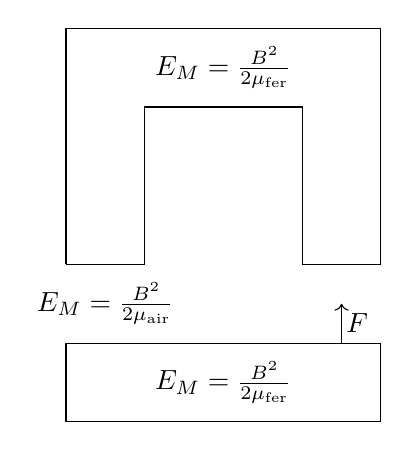
\begin{tikzpicture}\draw
      (0,1) |- (4,4) |- (3,1) |- (1,3) |- (0, 1)
      (0,0) rectangle (4, -1)
      (0.5,0.5) node{$E_M = \frac{B^2}{2\mu_\mathrm{air}}$}
      (3.7,0.25) node{$F$}
      (3.5,0) edge[->] (3.5,0.5)
      (2,3.5) node{$E_M = \frac{B^2}{2\mu_\mathrm{fer}}$}
      (2,-0.5) node{$E_M = \frac{B^2}{2\mu_\mathrm{fer}}$}
      ;
    \end{tikzpicture}
    \caption{Avant}
    \label{fig:before_portance}
  \end{subfigure}
  \begin{subfigure}{0.5\textwidth}
    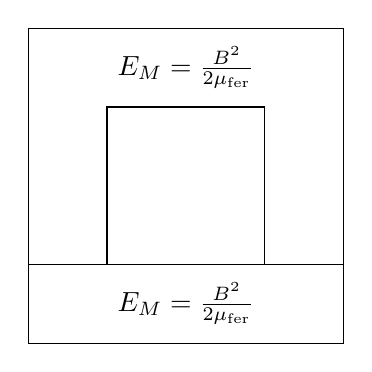
\begin{tikzpicture}\draw
      (0,1) |- (4,4) |- (3,1) |- (1,3) |- (0, 1)
      (0,1) rectangle (4, 0)
      (2,3.5) node{$E_M = \frac{B^2}{2\mu_\mathrm{fer}}$}
      (2,0.5) node{$E_M = \frac{B^2}{2\mu_\mathrm{fer}}$}
      ;
    \end{tikzpicture}
    \caption{Après}
    \label{fig:after_portance}
  \end{subfigure}
  \caption{Force portante avec 2 entrefers}
\end{figure}
On aimerait calculer $\vec F$, la force portante magnétique.
On utilise pour ça la loi de la conservation de l'énergie.
De la \figuref{before_portance} : la \figuref{after_portance},
on perd l'énergie magnétique contenue dans l'air,
c'est à dire
\[ 2Sd\frac{B^2}{2\mu_\mathrm{air}}. \]
Seulement, un travail a été fourni par la force portante magnétique $\vec F$,
il vaut
\[ W = Fd. \]
En égalisant les deux énergies, on trouve
\[ F = \frac{B^2S}{\mu_\mathrm{air}}. \]
S'il n'y a qu'un seul entrefer, et qu'il est dans le vide, $F$ devient
\[ F = \frac{B^2S}{2\mu_0}. \]

Dans un électroaimant avec entrefer,
Le flux reste constant y compris dans l'entrefer.
\[ \Phi_B = \text{constante} = BS. \]
Mais comme le $\mu_r$ est bien plus petit que le $\mu_r$ du matériau
et que $B = \mu_0\mu_r H$,
$H$ de l'entrefer est bien plus grand que $H$ du matériau.
\[ {\mu_r}_e \ll {\mu_r}_m \Rightarrow H_e \gg H_m. \]

Dans un électroaimant avec entrefer,
tout le champ magnétisant $H$ se retrouve dans l'entrefer.
Comme, $H_m$ est petit,
il est impossible de magnétiser complètement le
matériau à saturation quand il a un entrefer.
Tout le champ se retrouve donc dans l'entrefer.
Cela explique la démagnétisation des aimants permanents ouverts.


\section{Équations de Maxwell}
La relation entre champs électriques et magnétiques et
leurs sources peut être énoncé en 4 équations.
On les appelle les équations de Maxwell.

Lois de Gauss
\begin{align*}
  \oiint \E \cdot \dif \vec S &= \frac{Q_\mathrm{encl}}{\perm_0\perm_r}
  = \frac{1}{\perm_0\perm_r}\iiint \rho \dif V\\
  \oiint \B \cdot \dif \vec S &= 0.
\end{align*}
Loi d'Ampère
% Faut pas rajouter \perm_r dans celle-ci ?
\[ \oint \B \cdot \dif \vec l =
\mu_0\mu_r \left(I_\mathrm{C} + \perm_0\perm_r \frac{\dif \Phi_E}{\dif t}\right). \]
%= \mu_0\mu_r \iint \vec J \cdot \dif \vec S \]
Loi de Lenz-Faraday
\[ \oint \E \cdot \dif \vec l = \EMF = - \frac{\dif \Phi_B}{\dif t}
= - \frac{\dif}{\dif t}\int \B \dif \vec S. \]

\part{Magnétisme dans la matière}
Soit $H$, le champ magnétique ou magnétisant.
C'est le champ extérieur,
ce n'est pas encore le champ présent dans le matériau.
$B$ est le champ magnétique ou induction magnétique.
C'est le champ qui est ressenti dans le matériau.
Il est induit par un certain champ magnétique $H$.

Pour passer de $H$ à $B$,
il faut savoir qu'un matériau,
sous un champ magnétique $H$, se magnétise.
On note la magnétisation $M$.
On sait maintenant écrire
\[ B = \mu_0 (H + M). \]

On définit aussi $\mu_r = 1 + \chi$ tels que
\[ B = \mu_0\mu_r H = \mu_0 (H + \chi H). \]

Il y a 3 types de magnétisme: diamagnétisme, paramagnétisme et ferromagnétisme.

$\mu_r$ et $\chi$ sont constants pour les matériaux diamagnétiques et
paramagnétiques mais pour les ferro ou ferrimagnétiques,
$B$ n'est pas proportionnel à $H$ donc
$\mu_r$ et $\chi$ ne sont \textbf{pas constants} !

Dans le vide, $M = 0$ et $\chi = 0$ donc $\mu_r = 1$ et $B = \mu_0 H$.

On note parfois $B_0 = \mu_0 H$,
l'induction magnétique qu'il y aurait dans le vide pour un certain $H$.

On définit aussi souvent $\mu = \mu_0 \mu_r$.

Un utilise les appellations suivantes
\begin{center}
  \begin{tabular}{ll}
    Susceptibilité magnétique & $\chi$\\
    Perméabilité magnétique du vide & $\mu_0$\\
    Perméabilité magnétique relative & $\mu_r$\\
    Perméabilité magnétique & $\mu$
  \end{tabular}
\end{center}

\section{Diamagnétisme}
Presque tous les matériaux sont diamagnétiques jusqu'à un certain point
(i.e. un certain $H$), même les matériaux paramagnétiques et ferromagnétiques.
C'est parce qu'un moment magnétique peut être induit dans la plupart
des atomes quand ils sont placés dans un champ magnétique.
Ce moment magnétique induit est antiparallèle au champ magnétique externe.
La somme de ces faibles moments magnétiques donne au matériau
un très faible champ magnétique $M$ antiparallèle au champ magnétique externe.
Pour des matériaux diamagnétiques, $\mu_r$ est très proche de l'unité tout en
lui étant inférieure.
Ce champ disparait quand le champ magnétique externe disparait.


\section{Paramagnétisme}
Quand un matériau paramagnétique est placé dans un champ magnétique,
le champ aide les moments magnétiques des atomes à s'alligner.
Ça produit un champ magnétique $M$ dans le matériau
qui est parallèle au champ appliqué. Pour des matériaux paramagnétiques,
$1.00001 \leq \mu_r \leq 1.003$.
Ce champ disparait quand le champ magnétique externe disparait.

\section{Ferromagnétisme}
\label{sec:ferro}
Dans un ferromagnétique, il y a formation de domaines magnétiques.
Dans ces domaines, les moments dipolaires sont tous alignés dans le même sens.
Les parois entre ces domaines sont appelées les parois de Bloch.
Lorsque $H$ augmente,
les domaines tendent à se fusionner pour finalement
n'en former plus qu'un qui est parallèle à $H$.
Dans ce cas, $M$ est à saturation, on le note $M_s$.
Pour les matériaux ferromagnétiques, $1000 \leq \mu_r \leq 100000$.

\subsection{Courbes d'hystérésis}
Pour un matériau ferromagnetique, on a $H \ll M$ donc on peut approximer
\[ B \approx \mu_0 M. \]
C'est pourquoi, dans beaucoup de courbes d'hystérésis,
on met $B$ en ordonnée alors que ça devrait être $M$.
C'est parce qu'on néglige le terme $\mu_0 H$ de $B = \mu_0 H + \mu_0 M$.

$M_s$ est l'aimantation à saturation.
On a
\[ M_s = n_B N \]
où $n_B$ est le moment magnétique résultant par atome
et $N$ est le nombre d'atomes par unité de volume.

$M_r$ est l'aimantation rémanante,
c'est à dire l'aimantation restante si on retire le champ magnétique
extérieur après avoir aimanté le matériau à saturation.

$H_c$ est le champ coercitif, c'est, en valeur absolue,
le champ magnétique extérieur nécessaire pour désaimanter
un matériau ayant été aimanté à saturation.

\subsection{Matériaux magnétiques doux et durs}
Les ferromagnétiques durs ont une courbe d'hystérésis plus large et
nécessitent donc plus d'énergie pour
être magnétisés/démagnétisés que les ferromagnétiques doux.
Par contre leur $H_c$ est plus important,
ce sont donc de meilleur aimant permanent alors que
les magériaux magnétiques doux sont des meilleurs transformateurs.

Les matériaux magnétiques durs ont une plus importante
résistance au déplacement des parois de Bloch.

\section{Détermination de type de magnétisation}
Dans un atome, chaque électron engendre deux moments magnétiques
\begin{description}
  \item[Moment magnétique orbital]
    Moment magnétique résultant de la révolution de
    l'électron autour d'un noyau (comme un courant dans une boucle).
  \item[Moment magnétique de spin]
    Moment magnétique résultant de l'électron tournant sur lui-même.
\end{description}
\begin{itemize}
  \item Si la somme de ces moments est nulle,
    le matériau est \textbf{diamagnétique};
  \item Sinon, si les atomes adjacents du matériau n'interagissent pas
    ensemble pour produire des moments dont la somme contribue
    à leur alignement, il est \textbf{paramagnétique};
  \item Sinon, cette interaction permettra de garder un champ magnétique
    rémanent $B_r$ en l'absence de champ extérieur.
    \begin{itemize}
      \item Si dans le matériau,
        la géométrie est telle que les moments magnétiques des différents
        atomes vont s'annuler,
        il est soit \textbf{antiferromagnétique} s'ils s'annulent complêtement,
        soit \textbf{ferrimagnétique} dans le cas contraire;
      \item Sinon, il est \textbf{ferromagnétique}.
    \end{itemize}
    L'aimantation à saturation est plus forte pour
    les matériaux ferromagnétiques.
\end{itemize}
Notons qu'à partir d'une certaine température $T_c$,
propre a chaque matériau,
appelée température de Curie, les forces produisant l'alignement mutuel
des moments de spin s'annulent.
Les matériaux ferro ou ferrimagnétiques deviennent alors paramagnétiques.

%FIXME: find a place for the following information
Si on place une ferrite à l'intérieur d'une bobine,
l'entièreté du $\B$ se retrouvera dans la ferrite,
le $\B_{ext}$ est considéré comme nul.

\section{Superconductivité}
Certains matériaux sont des superconducteurs.
Ils ont une température critique $T_c$ qui varie d'un matériau à l'autre.
Pour chaque température $T < T_c$,
il existe un champ magnétique critique $H_c(T)$ tel que
pour tout $H < H_c(T)$, le matériau soumis à un champ magnétique externe $H$
à une température $T$ est en phase superconductrice
(voir \figuref{tbc}).

$H_c(T)$ est décroissant.
À une certaine température $T > T_c$, quelle que soit le champ magnétique $H$,
le matériau sera en phase normale (voir \figuref{tbc}).

Si un matériau est en phase superconductrice,
$B = 0$ à l'intérieur du matériau, c'est à dire que $M = -H$.
On appelle ça l'\emph{effet Meissner}.

Ça a aussi pour effet de rapprocher les lignes de champ magnétique extérieures
plus proche les unes des autres lorsqu'elle sont proche du matériau.
C'est à dire que $B$ augmente.

En phase normale, $B = \mu_r \mu_0 H$ à l'intérieur du matériau.
%$B \approx \mu_0 H$ à l'intérieur du matériau.
% <- Why ? Only para or dia are super ? See young p.980 édition 13 chap 29

\begin{figure}
  \begin{center}
    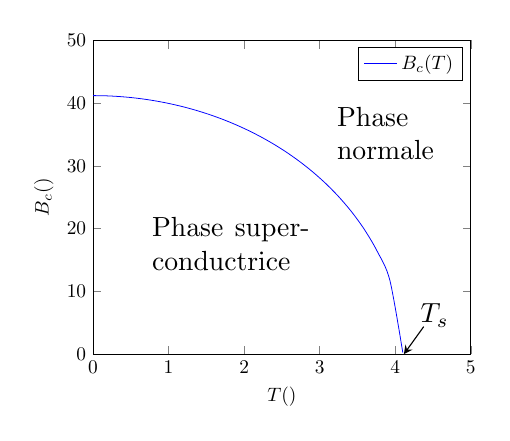
\begin{tikzpicture}[scale=0.7]
      \begin{axis}[xmin=0,xmax=5,ymin=0,ymax=50,
        xlabel=$T(\kelvin)$, ylabel=$B_c(\milli\tesla)$]
        %\xlabel{$T$}
        \addplot[smooth, color=blue, domain=0:4.1] {41.2*sqrt(1 - (x/4.1)^2)};
        \addlegendentry{$B_c(T)$}
      \end{axis}
    \node at (2.5, 2)
      {\begin{minipage}{2cm}Phase superconductrice\end{minipage}};
    \node at (5.5, 4) {\begin{minipage}{1.5cm}Phase normale\end{minipage}};
      \draw[style=-stealth] (6, 0.5) to (5.64, 0);
      \node at (6.2, 0.7) {$T_s$};
    \end{tikzpicture}
  \end{center}
  \caption{Relation entre $T$ et $B_c$ pour le mercure pur}
  \label{fig:tbc}
\end{figure}

\annexe
L'annexe est consituée de raisonnements intéressants
faisant des liens avec différentes matières.
Leur contenu ne fait pas partie de la matière.
\section{Explication de la loi de Gauss}
\label{ann:gauss}
Par le théorème de la divergence, on a
\[ \Phi = \oiint \B \cdot \dif \vec S = \iiint \newdiv \B \cdot \dif V. \]
Seulement, on a $\newdiv \B = 0$ qui est dû au fait
qu'il n'existe pas de monopôle magnétique.
D'où $\Phi = 0$.

Pour $\E$, on a $\newdiv \E = \frac{\rho}{\perm_0}$.
Où $\rho$ est la densité de charge par unité de volume.
D'où $\Phi = \frac{Q_\mathrm{int}}{\perm_0}$.

\end{document}
